\documentclass[12pt]{article} %style de document
%utilisation du squelette latex de cours de l'an dernier
\usepackage[utf8]{inputenc} %encodage des caractères
\usepackage[french]{babel} %paquet de langue français
\usepackage[T1]{fontenc} %encodage de la police
\usepackage[top=2cm,bottom=2cm,left=2cm,right=2cm]{geometry} %marges
\usepackage{graphicx} %'affichage des images
\frenchbsetup{StandardLists=true}
\usepackage{enumitem}
\usepackage{amssymb}
\usepackage{fancyhdr}
\usepackage{graphicx}
\usepackage{dsfont}
\usepackage{upgreek}


\pagestyle{fancy}
\usepackage{xcolor} %ajouter couleur de fond
\definecolor{white}{RGB}{255,255,255}
\pagecolor{white}

\usepackage{cite}


\usepackage{verbatim}

\usepackage{hyperref}

%supprimer le trait du header
\renewcommand\headrulewidth{0pt}

%supprimer les endroits de footeur et header que l'on ne veut pas
\fancyfoot[L]{}
\fancyfoot[R]{}

\fancyhead[L]{}



\begin{document} %début du document
\begin{center}


\section*{Rapport projet M1 Hacking éthique}

Titouan LE BRET

Elouan MOELLO

M1 Cybersécurité

\bigskip


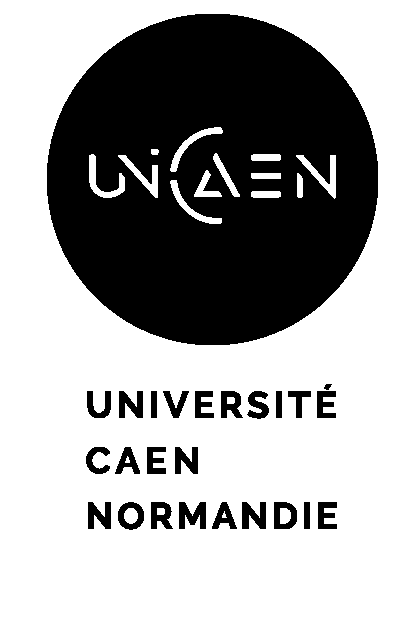
\includegraphics[scale=1.2]{images/LogoUNICAEN}
\begin{figure}[!h]
\label{}
\end{figure}
\end{center}



\newpage

\renewcommand{\contentsname}{Sommaire}
\tableofcontents




\newpage



\section{Introduction}
	\subsection{Présentation générale du projet}
		Contexte : réalisation d’un projet collaboratif dans le cadre du Master 1 Cybersécurité.
Explication des deux volets :
\begin{enumerate}
    \item Un site web avec Django axé sur la gestion sécurisée des inscriptions à une course, incluant des paiements en ligne et des protections des données utilisateurs.
    \item Une application Rust RSA pour approfondir les aspects de la cybersécurité, notamment la création et la validation de clés RSA.

\end{enumerate}
	
			
		
	\subsection{Organisation du projet}
		Rôles de chaque participant dans le développement des deux projets.
		Diagramme de gant (voir diapo)
	



\section{Conception générale}
	\subsection{Vision globale des deux projets}
		Les projets sont indépendants techniquement tout en ayant une base conceptuelle commune dans la cybersécurité.
        \begin{itemize}
            \item Site Django : Gestion sécurisée des inscriptions et des paiements.
            \item Application Rust RSA : Exploration et validation d'algorithmes cryptographiques.
        \end{itemize}

	
	\subsection{Cahier des charges}
		\textbf{Site Django :}
        \begin{itemize}
            \item Gestion des inscriptions utilisateur (création de compte, connexion via OAuth2).
            \item Paiements sécurisés en ligne.
            \item Sécurisation des fichiers téléchargés par les participants (PDF).
            \item Protection contre les attaques (exemple : reCAPTCHA).
        \end{itemize}
        \textbf{Application Rust RSA :} 
        \begin{itemize}
            \item Génération et validation de clés RSA.
            \item Tests de vulnérabilité des clés (taille insuffisante, non-primalité).
        \end{itemize}

	\subsection{Contraintes et exigences}
		\begin{enumerate}
		    \item \textbf{Sécurité} : Éviter les vulnérabilités (XSS, injections SQL pour Django, attaques par timing pour RSA).
            \item \textbf{Performance} : Réponse rapide du site web et efficacité des calculs cryptographiques.
            \item \textbf{Adaptabilité} : Modularité pour permettre des évolutions futures.

		\end{enumerate}


\section{Développement du site Django}
	\subsection{Fonctionnalités principales}
        Via django nous avons pu développer plusieurs fonctionnalités principales pour le projet web comme: l'inscription des utilisateurs, le paiement sécurisé via paypal, l'intégration avec OAuth2 (Google) et la sécurisation des fichiers pdf. Django permet d'implémenter une fonctionnalité administrateur, ce qui nous permet de voir les inscriptions et de les valider si toutes les informations sont correctes.


	\subsection{Approche technique}
		\subsubsection{Architecture Django :} 
            Django propose une architecture basée sur le model,view et templete.  Le dossier site course est le dossier principal, il contient le fichier setting.py qui permet de configurer les paramètres par défaut de notre application. Les autres dossiers sont des applications comme le dossiers inscriptions par exemple. Ce dossier contient des fichiers comme: \\
            - models.py:  Ce modèle stocke les informations relatives à l'inscription d'un participant à une course. \\ \\
            - view.py: Cette vue permet de faire le lien entre les tests des différentes fonctions comme l’inscription ou la suppression de l’inscription, et de faire l'appel des templetes via le fichier urls.py. Par exemple, plusieurs tests sont réalisés avant de valider l'inscription. \\ \\
            - signals.py: Ce fichier permet de gérer les signaux, par exemple lorsqu'un admin valide l’inscription d’un utilisateur, ce fichier reçoit un signal et envoie un mail de validation d'inscription à l’utilisateur grâce à une fonction.

            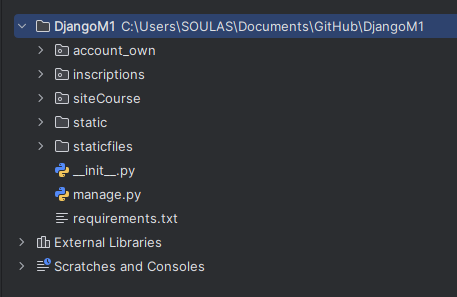
\includegraphics[scale=0.6]{images/Capture_structure.PNG}
            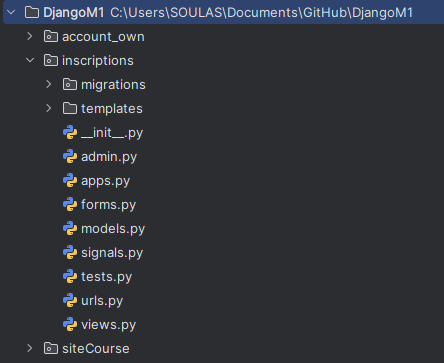
\includegraphics[scale=0.6]{images/Capture_structure-inscription.PNG}

        \subsubsection{Envoi d’e-mails :}
            Configuration de SendGrid pour des notifications fiables.\\
            L’envoi d’e-mails est utilisé dans plusieurs cas comme pour la création du compte ou pour la validation de l’inscription à une course. Voici un exemple de mail reçu lors de la validation d'une course par un administrateur.
    
            \begin{figure}[hbtp]
            \centering
            
\includegraphics[scale=0.8]{images/validationMAIL.PNG}
            \end{figure}

        \subsubsection{Protection des formulaires :}
            Chaque formulaires ont un Google reCAPTCHA qui permet de les sécuriser.
            \begin{figure}[hbtp]
            \centering
            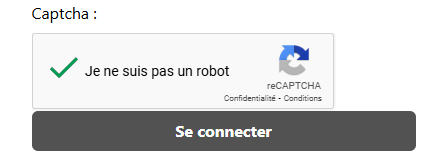
\includegraphics[scale=0.8]{images/Capture_captcha.PNG}
            \end{figure}
            
        \subsubsection{Partie administrateurs :}
            Comme évoqué précédemment nous avons une partie administrateurs qui permet de gérer toutes les inscriptions. Nous pouvons voir toutes les informations de l'utilisateur ainsi que les documents pdf importés, ce qui nous permet de vérifier la validité de celui-ci. Il y a aussi un case qui est cochée ou non si le paiement à été effectué et validé. Si toute les informations sont correctes alors l'administrateur peut cocher une case “inscription complète” qui va valider l’inscription et envoyer un mail automatiquement.

            \begin{figure}[hbtp]
            \centering
            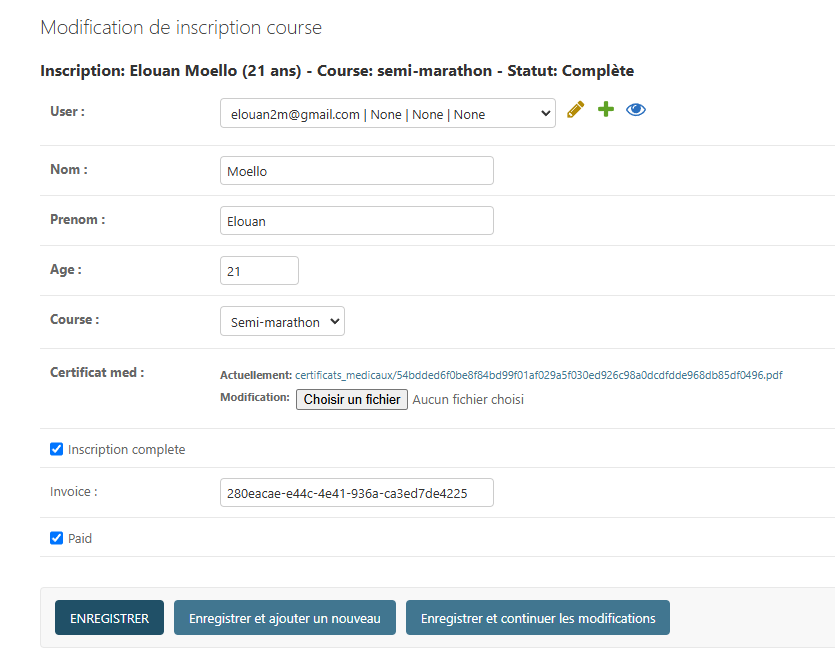
\includegraphics[scale=0.6]{images/admin_gestion.PNG}
            \end{figure}
            \newpage
        \subsubsection{ basse de données :}
            Chaque inscription est stockée dans une base de données avec toutes ses informations. Ces inscriptions ont toutes un identifiant unique qui permet de les différencier. Grâce à cette BDD nous pouvons récupérer les informations voulu.


		
		
	\subsection{Sécurisation du site}
        \begin{enumerate}
            \item \textbf{Validation des données :}\\ \\
                Contrôles sur les entrées utilisateur (taille, format, validation).
            \item \textbf{Protection des fichiers :}\\ \\
                Restrictions des téléchargements non authentifiés.
            \item \textbf{Sécurisation des paiements :}\\ \\
                Le paiement est effectué grâce à l'implémentation de paypal. Lorsque l'utilisateur complète son inscription, un lien vers l’api paypal lui permet de procéder au paiement. Si l'utilisateur annule le paiement, il pourra par la suite procéder au paiement sur la page d’inscription. Sur cette page toutes les inscriptions de l'utilisateur sont affichées et il peut procéder au paiement de chaque course si celle-ci n'est pas encore payée. Pour effectuer les tests de paiement nous avons créé deux comptes paypal en mode “sand box” (bac à sable). Ces comptes sont donc fictifs et permettent d'effectuer des tests de paiement. Nous avons donc:\\
                Un compte personnel qui permet d'effectuer les paiements.\\
                personal@etu.unicaen.fr\\
                mdp: motdepasseperso\\
                Un compte business qui récupère l’argent de chaque inscription.\\
                business@etu.unicaen.fr\\
                mdp: motdepassebusiness\\
                Nous pouvons consulter ces compte avec ce lien:\\  https://www.sandbox.paypal.com/fr/home\\

        \end{enumerate}


	\subsection{Problèmes rencontrés et solutions}
        \begin{enumerate}
            \item \textbf{Difficultés techniques :}\\\\
                Configuration de SendGrid : documentation approfondie et tests successifs.\\
                Gestion des fichiers : stockage local temporaire remplacé par des solutions cloud envisagées.

            \item \textbf{Communication HTTPS et local :}\\\\
                Une fois le paiement effectué, le serveur paypal envoie un “signal ipn” qui permet de récupérer les informations de paiement. Le problème est que la communication est effectuée en https alors que notre serveur est en local lors de la phase de développement. Donc pour récupérer ce signal nous avons utilisé un outil qui est “ngrok” qui permet de mettre notre application en https. Cet outil est provisoire pour la phase de test mais ce n’est pas celui-ci qui va nous permettre à terme de mettre notre site en https.\\
                Ngrok nous permet donc d’avoir un nouveau lien en https ce qui nous permet de récupérer le signal de paiement.\\ Voici la fenêtre de gestion Ngrok.


                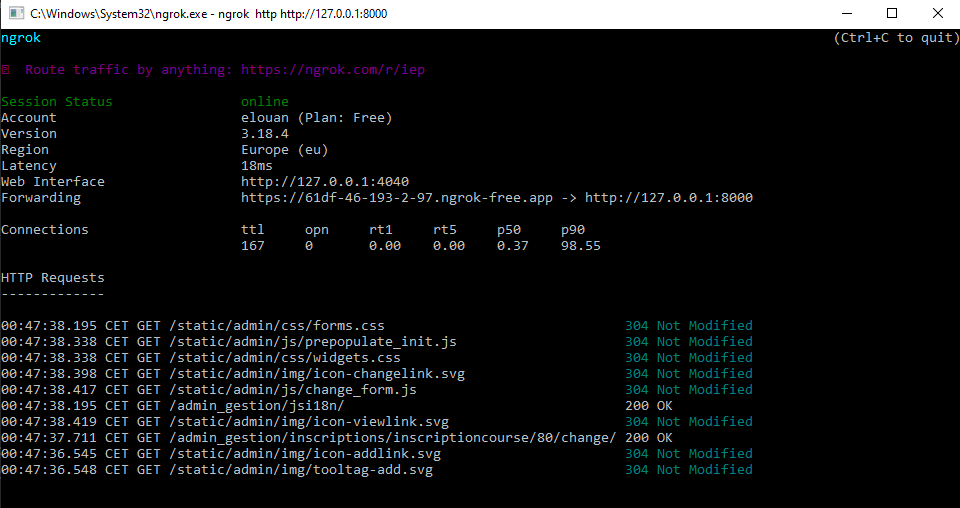
\includegraphics[scale=0.6]{images/Capture_M1Ngrok.PNG}

        \end{enumerate}
    


	\subsection{Axes d'améliorations}
		-Stockage des images en ligne (dans un DIsks sur render ou dans le CLoud google) -> demande abonnements payants \\\\
        \textbf{Paiements Stripe:}\\
            Un autre mode de paiement possible est le paiement par stripe. Il est tout aussi efficace que paypal, il intègre aussi une API. On peut dire qu’il est plus polyvalent que paypal, il intègre aussi plus de devise.
            Nous avons commencé à intégrer Stripe à notre projet web, mais vu le temps qu’il nous restait nous avons préféré nous concentrer sur la finalisation du projet.

		

	

\section{Développement de l'application Rust RSA}
	\subsection{Objectifs et fonctionnalités principales}
		Tester la sécurité des clés RSA (validité, erreurs courantes).
Générer et valider des clés publiques.

	\subsection{Organisation technique}
		Structure des modules Rust (mod.rs, gestion des entrées).
Utilisation de rsa::BigUint pour les calculs.
Gestion des événements d’entrée/sortie et affichage des résultats.

	\subsection{Problèmes rencontrés et solutions}
		Gestion des entrées sans utiliser de String.

	\subsection{Axes d’amélioratrions }
		-Ajout de fonctions toujours possibiles sur les 2 pages
		-Ajout de 2 pages pour tester la signatures RSA 



\section{Conclusion et perspectives}
	\subsection{Différences fondamentales}
		Objectifs distincts : site orienté utilisateur, application centrée sur la cryptographie.
Langages et environnements de développement (Python/Django vs Rust).


	\subsection{Apport de chaque projet dans le cadre de la cybersécurité}
		Impact du site : mise en œuvre des bonnes pratiques de sécurité web + apprentissage django et d’API.
Impact de l’application : exploration de la cryptographie RSA et apprentissage de RUST
	
	
	
	\subsection{Bilan global}
		Synthèse des apprentissages.
Des améliorations possibles (projets évolutifs)



\section*{Annexes}
	\subsection{Codes sources importants}
		Extraits des parties clés de Django et Rust.
	\subsection{Ressources externes}
		Bibliographies, articles, et outils utilisés





\end{document}
